% !TEX TS-program = pdflatex
% !TEX encoding = UTF-8 Unicode

% This is a simple template for a LaTeX document using the "article" class.
% See "book", "report", "letter" for other types of document.

\documentclass[11pt]{article} % use larger type; default would be 10pt

\usepackage[utf8]{inputenc} % set input encoding (not needed with XeLaTeX)

\setlength{\parindent}{2em}
\setlength{\parskip}{1em}

%%% Examples of Article customizations
% These packages are optional, depending whether you want the features they provide.
% See the LaTeX Companion or other references for full information.

%%% PAGE DIMENSIONS
\usepackage[margin=0.75in]{geometry}
\usepackage{geometry} % to change the page dimensions
\geometry{a4paper} % or letterpaper (US) or a5paper or....
% \geometry{margin=2in} % for example, change the margins to 2 inches all round
% \geometry{landscape} % set up the page for landscape
%   read geometry.pdf for detailed page layout information

\usepackage{graphicx} % support the \includegraphics command and options

% \usepackage[parfill]{parskip} % Activate to begin paragraphs with an empty line rather than an indent

%%% PACKAGES
\usepackage{booktabs} % for much better looking tables
\usepackage{array} % for better arrays (eg matrices) in maths
\usepackage{paralist} % very flexible & customisable lists (eg. enumerate/itemize, etc.)
\usepackage{verbatim} % adds environment for commenting out blocks of text & for better verbatim
\usepackage{subfig} % make it possible to include more than one captioned figure/table in a single float
\usepackage{pgfplots}
\usepackage{indentfirst}
\usepackage{bm}
\usepackage{todonotes}
\usepackage{mathtools}
\usepackage{amssymb}
\usepackage{amsmath}
\usepackage{graphics}
\usepackage{hyperref}
\usepackage{fontawesome}
\usepackage{enumitem}
\usepackage{tkz-graph}
\tikzset{
  LabelStyle/.style = { font = \bfseries },
  VertexStyle/.append style = { inner sep=5pt, font = \bfseries},
  EdgeStyle/.append style = { -> } }
\setlist{nosep}
% These packages are all incorporated in the memoir class to one degree or another...

%%% HEADERS & FOOTERS
\usepackage{fancyhdr} % This should be set AFTER setting up the page geometry
\pagestyle{fancy} % options: empty , plain , fancy
\renewcommand{\headrulewidth}{0pt} % customise the layout...
\lhead{}\chead{}\rhead{}
\lfoot{}\cfoot{\thepage}\rfoot{}

%%% SECTION TITLE APPEARANCE
\usepackage{sectsty}
\allsectionsfont{\sffamily\mdseries\upshape} % (See the fntguide.pdf for font help)
% (This matches ConTeXt defaults)

%%% ToC (table of contents) APPEARANCE
\usepackage[nottoc,notlof,notlot]{tocbibind} % Put the bibliography in the ToC
\usepackage[titles,subfigure]{tocloft} % Alter the style of the Table of Contents
\renewcommand{\cftsecfont}{\rmfamily\mdseries\upshape}
\renewcommand{\cftsecpagefont}{\rmfamily\mdseries\upshape} % No bold!

 %%% END Article customizations

%%% The "real" document content comes below...

\title{Using the Fundamental Theorem of Linear Algebra}
\author{Dale Kim\\Insomniac Games, Inc.\\\href{mailto:dkim@insomniacgames.com}{dkim@insomniacgames.com} \\\faTwitter \href{https://twitter.com/roflraging}{@Roflraging}}
%\date{} % Activate to display a given date or no date (if empty),
         % otherwise the current date is printed 

\begin{document}
\maketitle

\section{Application}
Previously, I went over the Fundamental Theorem of Linear Algebra and
the relationships it describes between the different spaces.  One of
the key ideas of the theorem is orthogonality, which is a very simple
but powerful tool when applying linear algebra to real problems.  This
article will show some ways the theorem and orthogonality can be used
to your advantage.

\section{A simple example}
Consider the task of determining if a given column vector $\bm{b}$ is
in the column space of A.  One method of figuring this out would be to
attempt to solve $\bm{Ax}$ = $\bm{b}$ and see if a solution exists.
This is a valid approach, but what if you were given multiple
$\bm{b}$'s?  You would not want to solve the whole system for each
$\bm{b}$.

With orthogonality, you can easily determine the answer to this
question for any $\bm{b}$.  Recall that $\bm{C(A)}\perp\bm{N(A^T)}$ by
the Fundamental Theorem of Linear Algebra.  We know that any vector
$\bm{b}$ that is in $\bm{C(A)}$ must be orthogonal to any vector in
$\bm{N(A^T)}$.  In other words, if $\bm{b}$ is orthogonal to the basis
vectors that make up the left nullspace, then it must be in the column
space.  All that is required is the complete solution to the left
nullspace of A, which is easily obtained via elimination.

The key realization here is that you can make determinations about
\textit{all} vectors $\bm{b}$ through properties of $\bm{A}$ alone.
There is no need to have a particular $\bm{b}$ to solve for.

\section{Circuit design}
The previous problem is, perhaps, too much of a toy example to show
the importance of orthogonality.  A better example is circuit design
(and more broadly, network flow).  In circuit design, you may wish to
take a set of nodes (junctions) with some description of their
connectivity and determine voltages to achieve a desired current.

\begin{center}
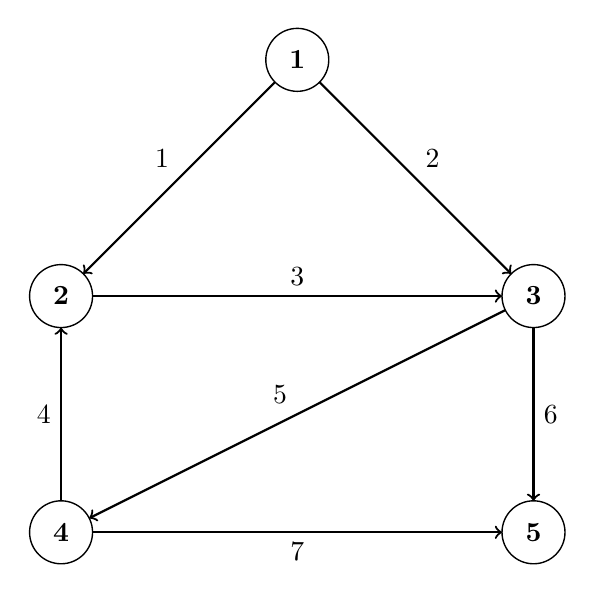
\begin{tikzpicture}
  \SetGraphUnit{3}
  \Vertex{1}
  \SOWE(1){2}
  \SOEA(1){3}
  \SO(2){4}
  \SO(3){5}
  \tikzstyle{LabelStyle}=[above left] \Edge[label = 1](1)(2)
  \tikzstyle{LabelStyle}=[above right] \Edge[label = 2](1)(3)
  \tikzstyle{LabelStyle}=[above]\Edge[label = 3](2)(3)
  \tikzstyle{LabelStyle}=[left] \Edge[label = 4](4)(2)
  \tikzstyle{LabelStyle}=[above left] \Edge[label = 5](3)(4)
  \tikzstyle{LabelStyle}=[right] \Edge[label = 6](3)(5)
  \tikzstyle{LabelStyle}=[below] \Edge[label = 7](4)(5)
\end{tikzpicture}
\[
\bm{A} = \begin{bmatrix*}[r]
  -1 & 1 & 0 & 0 & 0 \\
  -1 & 0 & 1 & 0 & 0 \\
   0 & -1 & 1 & 0 & 0 \\
   0 & 1 & 0 & -1 & 0 \\
   0 & 0 & -1 & 1 & 0 \\
   0 & 0 & -1 & 0 & 1 \\
   0 & 0 & 0 & -1 & 1
\end{bmatrix*}
\]
\end{center}

Above is a circuit with five nodes and seven directed edges which
describe how the nodes are connected to each other.  $\bm{A}$ is the
adjacency matrix where each row $i$ corresponds to the edge labeled
$i$.  The column $j$ represents node $j$ and the entries $-1$ and $1$
in a row indicate the edge begins and ends, respectively, at the
corresponding nodes.  In the problem $\bm{Ax}$ = $\bm{b}$, $\bm{x}$
represents the voltage at each node and $\bm{b}$ is the voltage
difference across each edge.

\[
\bm{Ax} = \begin{bmatrix*}[r]
  -1 & 1 & 0 & 0 & 0 \\
  -1 & 0 & 1 & 0 & 0 \\
   0 & -1 & 1 & 0 & 0 \\
   0 & 1 & 0 & -1 & 0 \\
   0 & 0 & -1 & 1 & 0 \\
   0 & 0 & -1 & 0 & 1 \\
   0 & 0 & 0 & -1 & 1
\end{bmatrix*}
\begin{bmatrix} \bm{x_1} \\ \bm{x_2} \\ \bm{x_3} \\ \bm{x_4} \\ \bm{x_5} \end{bmatrix} =
\begin{bmatrix} x_2 - x_1 \\ x_3 - x_1 \\ x_3 - x_2 \\ x_2 - x_4 \\ x_4 - x_3 \\ x_5 - x_3 \\ x_5 - x_4 \end{bmatrix} = \bm{b}
\]

If you wanted to find the set of all voltages which have a zero
voltage difference, you simply solve for $\bm{Ax} = \bm{0}$, the
nullspace!  In this matrix, we have a relatively boring nullspace
solution of $(v, v, v, v, v)$, which says that if all nodes have the
same voltage, no voltage difference is present.

\[
\bm{A^T} = \begin{bmatrix*}[r]
  -1 & -1 & 0 & 0 & 0 & 0 & 0 \\
  1 & 0 & -1 & 1 & 0 & 0 & 0 \\
  0 & 1 & 1 & 0 & -1 & -1 & 0 \\
  0 & 0 & 0 & -1 & 1 & 0 & -1 \\
  0 & 0 & 0 & 0 & 0 & 1 & 1
\end{bmatrix*}
\]

$\bm{A^T}$ shows a different view where each row now represents a node
and the columns are edges.  Before, $\bm{Ax} = \bm{b}$ described
something about edges (the voltage difference), but $\bm{A^Ty} =
\bm{c}$ is something else:

\[
\bm{A^Ty} =
\begin{bmatrix*}[r]
  -1 & -1 & 0 & 0 & 0 & 0 & 0 \\
  1 & 0 & -1 & 1 & 0 & 0 & 0 \\
  0 & 1 & 1 & 0 & -1 & -1 & 0 \\
  0 & 0 & 0 & -1 & 1 & 0 & -1 \\
  0 & 0 & 0 & 0 & 0 & 1 & 1
\end{bmatrix*}
\begin{bmatrix} \bm{y_1} \\ \bm{y_2} \\ \bm{y_3} \\ \bm{y_4} \\ \bm{y_5} \\ \bm{y_6} \\ \bm{y_7} \end{bmatrix} =
\begin{bmatrix*}[r]
  -\bm{y_1} - \bm{y_2} \\
  \bm{y_1} + \bm{y_4} - \bm{y_3} \\
  \bm{y_2} + \bm{y_3} - \bm{y_5} - \bm{y_6} \\
  \bm{y_5} - \bm{y_4} - \bm{y_7} \\
  \bm{y_6} + \bm{y_7}
\end{bmatrix*} = \bm{c}
\]

The vector $\bm{y}$ represents current along the edges and $\bm{A^Ty}$
is the \textit{net current} (or flow) on each node.  What happens when
$\bm{c}$ is the zero vector?  It describes \emph{Kirchhoff's current
  law}, which says that for every node, current in must equal current
out (or net current is zero).  The left nullspace provides the perfect
description of all the currents $\bm{y}$ that satisfy this law.  For
this fact to be useful to us, we need to combine it with $\bm{Ax}$:

\[
\bm{A^TAx} = \bm{0}
\]

This equation ties together the voltages of the nodes to the currents
between the nodes and ensures that it satisfies Kirchhoff's current
law. \footnote{This is actually a less general form of $\bm{A^TCAx} =
  \bm{f}$, where $\bm{C}$ is the diagonal ``conductance'' matrix and
  $\bm{f}$ is the external current applied to the circuit.}  It may
not be clear why this is necessary, but the Fundamental Theorem of
Linear Algebra provides an explanation.  $\bm{Ax}$ produces a vector
$\bm{b}$ that is in the column space, which by the theorem is
perpendicular to the left nullspace.  Doesn't this mean that all
$\bm{b}$'s satisfy Kirchhoff's current law?

No!  The theorem only says $\bm{y^Tb} = \bm{0}$ if $\bm{b}$ is in the
column space and $\bm{y}$ is in the left nullspace of A; it says
nothing about what $\bm{A^Ty}$ (or $\bm{A^TAx}$) will
be! \footnote{Try $\bm{x} = (1, 2, 3, 4, 5)$.}  So, $\bm{b}$ must be
in both the column space and left nullspace of A, which necessitates
that $\bm{x}$ come from the nullspace of A (only the zero vector can
be in both the column space and the left nullspace).

\begin{thebibliography}{9}
\bibitem{strang}
  Gilbert Strang.
  \textit{Introduction to Linear Algebra, 4th Edition.}
  Welleslely - Cambridge Press, Wellesley, Massachusetts, 2009.
\end{thebibliography}

\end{document}
